\section{What closed-loop labels cost}
\label{sec:cost}

\subsection{Against human annotation}

The 55 models from the dial sweep were trained, validated and tested entirely
inside their own labeller, and had never been scored against the expert labels the
dataset ships. Scoring them against the human required no new training.

We score by mosaic: one decision per source pixel, taken by majority vote of the
crops covering it, compared once against the expert label. Patch scoring would count
each pixel about sixteen times and would hand the crop-dependent arms exactly the
reward this paper says patch scoring hands them, which would manufacture the result
rather than measure it.

\begin{figure}[tb]
\centering
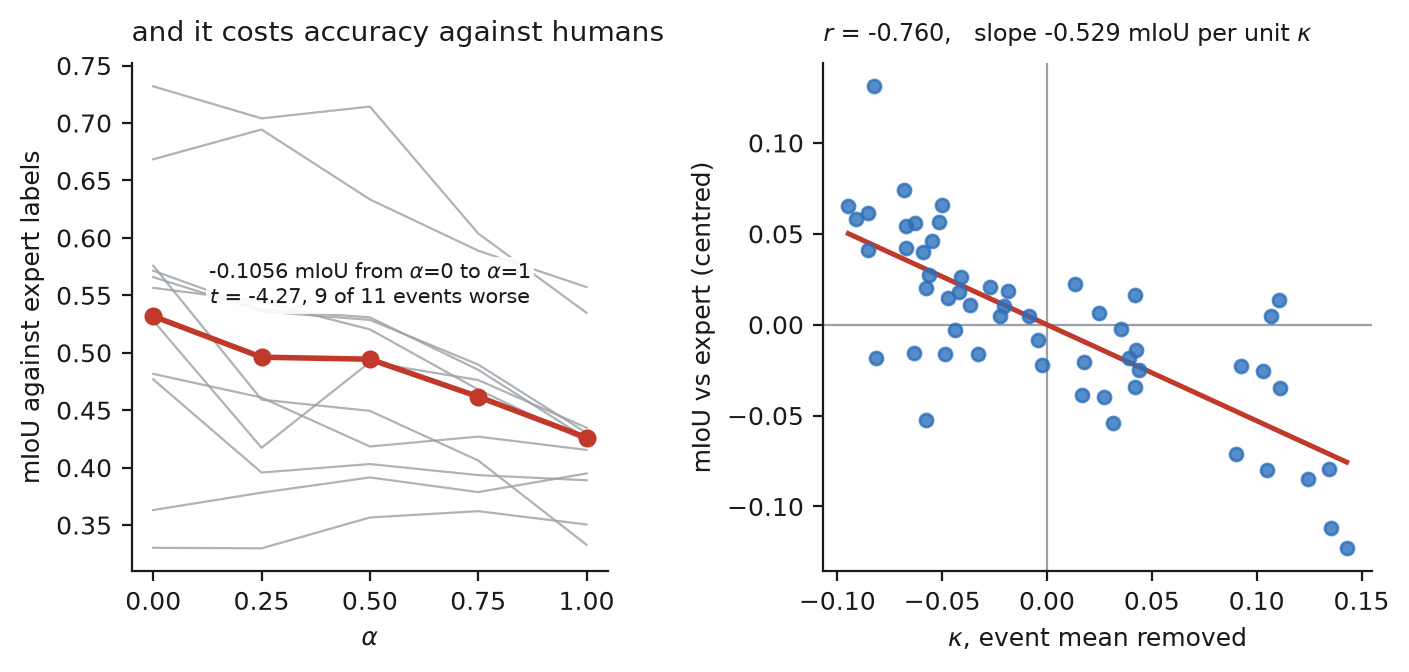
\includegraphics[width=\linewidth]{figures/shortcut_cost.png}
\caption{Left: mIoU against expert labels falls as the labeller becomes more
crop-dependent. Right: $\kap$ against that mIoU with each event's mean removed, so
the slope cannot come from events differing in difficulty.}
\label{fig:cost}
\end{figure}

\begin{table}[tb]
\centering
\small
\setlength{\tabcolsep}{3pt}
\begin{tabular}{lccccc}
\toprule
$\alpha$ & 0.00 & 0.25 & 0.50 & 0.75 & 1.00 \\
\midrule
mIoU vs expert & 0.5318 & 0.4962 & 0.4944 & 0.4618 & $\mathbf{0.4262}$ \\
\bottomrule
\end{tabular}
\caption{Accuracy against expert labels over the dial sweep of \cref{eq:dial},
mosaic scored.}
\label{tab:cost}
\end{table}

Accuracy against the expert labels falls monotonically with the dial
(\cref{tab:cost}). The cost of full crop-dependence is $-0.1056$ mIoU (sd $0.0821$,
$t = -4.27$), worse in 9 of 11 events. Pooled across the sweep with each event's
mean removed, $\kap$ tracks that loss at $r = -0.760$, a slope of $-0.529$ mIoU per
unit $\kap$ ($t = -8.50$), shown in the right panel of \cref{fig:cost}. Two events improve, by $+0.0318$ and $+0.0203$, both among the
lowest-mIoU events in the set. Absolute values are lower than this dataset's
whole-chip numbers because these are $128 \times 128$ crop-trained models with less
context; the quantity in use is the comparison across the dial, not the level.

\subsection{Is $\kap$ only a proxy for the dial?}

The dial moves $\kap$ and the damage together, so a correlation between them is
equally consistent with $\kap$ being a bystander. We therefore hold $\alpha$ fixed
and ask whether $\kap$ still separates events once the dial cannot vary.

\begin{table}[tb]
\centering
\small
\setlength{\tabcolsep}{3pt}
\begin{tabular}{lcccccc}
\toprule
$\alpha$ & 0.00 & 0.25 & 0.50 & 0.75 & 1.00 & mean \\
\midrule
$r$ & $-0.614$ & $-0.698$ & $-0.542$ & $-0.567$ & $-0.534$ & $\mathbf{-0.591}$ \\
\bottomrule
\end{tabular}
\caption{Correlation between $\kap$ and mIoU against expert labels, computed across
the eleven events separately at each dial setting.}
\label{tab:fixed}
\end{table}

All five settings give a negative correlation (\cref{tab:fixed}). Two are
individually significant at $n = 11$, the strongest at $p = 0.017$, and the other
three fall between $p = 0.069$ and $p = 0.091$. The five arms are not independent,
since the dial nests them by construction and they share the same eleven events, so
what the table shows is consistency across the sweep and not five separate tests. At
any fixed level of crop-dependence, the events where the model aligned more with the
crop labeller did worse against the human.

We do not claim $\kap$ is the mechanism by which the damage happens. That would need
a mediation design this experiment does not have. We claim it is an indicator that
survives removing the confound.
